\chapter{Исследовательская часть}

\section{Интерфейс приложения}

На рисункaх  \ref{fig:interface} -- \ref{fig:working1} приведено изображение интерфейса главного экрана приложения.
\FloatBarrier
\begin{figure}[h!]
	\centering{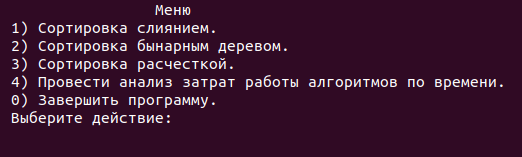
\includegraphics[scale=0.7]{photos/interface.png}}
	\caption{Интерфейс}
	\label{fig:interface}
\end{figure}
\FloatBarrier

Пользователь может ввести элементов массива вручную или автоматически, для которого необходимо упорядочить элементы по возростанию, а также выбрать метод, который будет использован для этого действия. 
В результате выводится отсортированный массив.
\FloatBarrier
\begin{figure}[h!]
	\centering{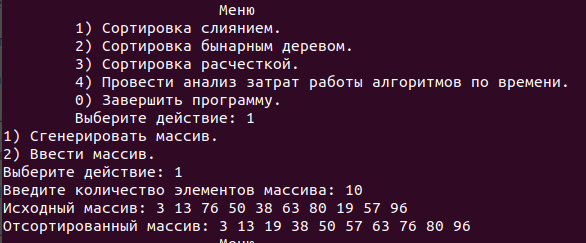
\includegraphics[scale=0.7]{photos/working.png}}
	\caption{Экран с результатом}
	\label{fig:working1}
\end{figure}
\clearpage

\section{Технические характеристики}

Технические характеристики устройства, на котором выполнялось тестирование:

\begin{itemize}
	\item операционная система: Ubuntu 22.04.3 LTS;
	\item оперативная память: 12 Гб;
	\item процессор: AMD® Athlon silver 3050u with radeon graphics × 2;
\end{itemize}

\section{Время выполнения реализаций алгоритмов}

На рисунке \ref{fig:graph1} приведено сравнение реализации всех алгоритмов сортировки в среднем случае, которые содержат 10, 20, 30, 40, 50, 100, 200, 300, 500, 1000 элементов.

\begin{figure}[ht!]
	\begin{center}
		\captionsetup{singlelinecheck = false, justification=centerfirst}
		\begin{tikzpicture}
			\begin{axis}[
				xlabel={Количество элементов в массиве},
				ylabel={Время в секундах},
				width = 0.95\textwidth,
				height=0.43\textheight,
				xmin=0, xmax=1000,
				ymode=log, 
				legend pos=north west,
				legend style={font=\footnotesize},
				xmajorgrids=true,
				grid style=dashed,
				]
				
				\addplot[
				blue,
				semithick,
				mark = *,
				mark size = 3pt,
				thick,
				] file {graph/merge.csv};
				
				\addplot[
				red,
				semithick,
				mark = *,
				] file {graph/bin_tree.csv};
				
				\addplot[
				green,
				semithick,
				mark = *,
				] file {graph/coctail.csv};
				
				\legend{
					Сортировка слиянием,
					Сортировка бинарным деревом,
					Сортировка расчесткой
				}
			\end{axis}
			
		\end{tikzpicture}
		\centering
		\caption{Сравнение времени работы реализаций алгоритмов}
		\label{fig:graph1}
	\end{center}
\end{figure}
\clearpage

На рисунке \ref{fig:graph2} приведено сравнение реализации всех алгоритмов сортировки в лудшем случае, которые содержат 10, 20, 30, 40, 50, 100, 200, 300, 500, 1000 элементов.

\begin{figure}[ht!]
	\begin{center}
		\captionsetup{singlelinecheck = false, justification=centerfirst}
		\begin{tikzpicture}
			\begin{axis}[
				xlabel={Количество элементов в массиве},
				ylabel={Время в секундах},
				width = 0.95\textwidth,
				height=0.43\textheight,
				xmin=0, xmax=1000,
				ymode=log, 
				legend pos=north west,
				legend style={font=\footnotesize},
				xmajorgrids=true,
				grid style=dashed,
				]
				
				\addplot[
				blue,
				semithick,
				mark = *,
				mark size = 3pt,
				thick,
				] file {graph/merge_best.csv};
				
				\addplot[
				red,
				semithick,
				mark = *,
				] file {graph/bin_tree_best.csv};
				
				\addplot[
				green,
				semithick,
				mark = *,
				] file {graph/coctail_best.csv};
				
				\legend{
					Сортировка слиянием,
					Сортировка бинарным деревом,
					Сортировка расчесткой
				}
			\end{axis}
			
		\end{tikzpicture}
		\centering
		\caption{Сравнение времени работы реализаций алгоритмов}
		\label{fig:graph2}
	\end{center}
\end{figure}
\clearpage

На рисунке \ref{fig:graph3} приведено сравнение реализации всех алгоритмов сортировки в худшем случае, которые содержат 10, 20, 30, 40, 50, 100, 200, 300, 500, 1000 элементов.

\begin{figure}[ht!]
	\begin{center}
		\captionsetup{singlelinecheck = false, justification=centerfirst}
		\begin{tikzpicture}
			\begin{axis}[
				xlabel={Количество элементов в массиве},
				ylabel={Время в секундах},
				width = 0.95\textwidth,
				height=0.43\textheight,
				xmin=0, xmax=1000,
				ymode=log, 
				legend pos=north west,
				legend style={font=\footnotesize},
				xmajorgrids=true,
				grid style=dashed,
				]
				
				\addplot[
				blue,
				semithick,
				mark = *,
				mark size = 3pt,
				thick,
				] file {graph/merge_worst.csv};
				
				\addplot[
				red,
				semithick,
				mark = *,
				] file {graph/bin_tree_worst.csv};
				
				\addplot[
				green,
				semithick,
				mark = *,
				] file {graph/coctail_worst.csv};
				
				\legend{
					Сортировка слиянием,
					Сортировка бинарным деревом,
					Сортировка расчесткой
				}
			\end{axis}
			
		\end{tikzpicture}
		\centering
		\caption{Сравнение времени работы реализаций алгоритмов}
		\label{fig:graph3}
	\end{center}
\end{figure}
\clearpage

\section{Используемая память}
На рисунке \ref{fig:graph4} приведено сравнение реализации всех алгоритмов сортировки по памяти, которые содержат 10, 20, 30, 40, 50, 100, 200, 300, 500, 1000 элементов.
\begin{figure}[ht!]
	\begin{center}
		\captionsetup{singlelinecheck = false, justification=centerfirst}
		\begin{tikzpicture}
			\begin{axis}[
				xlabel={Количество элементов в массиве},
				ylabel={Память в байтах},
				width = 0.95\textwidth,
				height=0.5\textheight,
				xmin=0, xmax=1000,
				ymode=log, 
				legend pos=north west,
				legend style={font=\footnotesize},
				xmajorgrids=true,
				grid style=dashed,
				]
				
				\addplot[
				blue,
				semithick,
				mark = *,
				mark size = 3pt,
				thick,
				] file {graph/merge_memory.csv};
				
				\addplot[
				red,
				semithick,
				mark = *,
				] file {graph/bin_tree_memory.csv};
				
				\addplot[
				green,
				semithick,
				mark = *,
				] file {graph/coctail_memory.csv};
				
				\legend{
					Сортировка слиянием,
					Сортировка бинарным деревом,
					Сортировка расчесткой
				}
			\end{axis}
			
		\end{tikzpicture}
		\centering
		\caption{Сравнение размеров реализаций алгоритмов в байтах}
		\label{fig:graph4}
	\end{center}
\end{figure}
\clearpage

\section*{Вывод}

В данном разделе проведено сравнение времени выполнения и использования памяти алгоритмов сортировки для массивов различного размера. 
Помимо оценки скорости выполнения, изучили, как каждый из алгоритмов влияет на использование памяти. 
В массивах до 50 элементов из графика \ref{fig:graph1} видно, что алгоритм сортировки бинарным деревом в среднем случае медленее работает чем алгоритм соритовки расчесткой. 
Такой результат получисля потому, что бинарное дерево не находится ближе к сбалансированнному состоянию, что ухудшает его производительность.

Наименее затратным по памяти оказался алгоритм сортировки расчесткой из-за того, что он использует только структуру массива, пока остальные алгоритмы используют дополнительные структуры.

